%; whizzy chapter
% -initex iniptex -latex platex -format platex -bibtex jbibtex -fmt fmt
% 以上 whizzytex を使用する場合の設定。


%     Tokyo Debian Meeting resources
%     Copyright (C) 2009 Junichi Uekawa
%     Copyright (C) 2009 Nobuhiro Iwamatsu

%     This program is free software; you can redistribute it and/or modify
%     it under the terms of the GNU General Public License as published by
%     the Free Software Foundation; either version 2 of the License, or
%     (at your option) any later version.

%     This program is distributed in the hope that it will be useful,
%     but WITHOUT ANY WARRANTY; without even the implied warranty of
%     MERCHANTABILITY or FITNESS FOR A PARTICULAR PURPOSE.  See the
%     GNU General Public License for more details.

%     You should have received a copy of the GNU General Public License
%     along with this program; if not, write to the Free Software
%     Foundation, Inc., 51 Franklin St, Fifth Floor, Boston, MA  02110-1301 USA

%  preview (shell-command (concat "evince " (replace-regexp-in-string "tex$" "pdf"(buffer-file-name)) "&"))
% 画像ファイルを処理するためにはebbを利用してboundingboxを作成。
%(shell-command "cd image200906; ebb *.png")

%%ここからヘッダ開始。

\documentclass[mingoth,a4paper]{jsarticle}
\usepackage{monthlyreport}

% 日付を定義する、毎月変わります。
% date --date 'third saturday'
\newcommand{\debmtgyear}{2009}
\newcommand{\debmtgmonth}{8}
\newcommand{\debmtgdate}{8}
\newcommand{\debmtgnumber}{55}

\begin{document}

\begin{titlepage}
\thispagestyle{empty}

% タイトルページ:編集必要な部分は最初のマクロに飛ばすこと

\vspace*{-2cm}
第\debmtgnumber{}回 東京エリア Debian 勉強会資料

\hspace*{-2.4cm}
\includegraphics[width=210mm]{image200801/2008title.eps}\\
\hfill{}\debmtgyear{}年\debmtgmonth{}月\debmtgdate{}日

\end{titlepage}

\dancersection{Introduction}{上川 純一}

\begin{multicols}{2}
 
 
 今月のDebian勉強会へようこそ。これからDebianの世界にあしを踏み入れると
 いう方も、すでにどっぷりとつかっているという方も、月に一回Debianについ
 て語りませんか?

 Debian勉強会の目的は下記です。

 \begin{itemize}
 \item \underline{Debian Developer} (開発者)の育成。
 \item 日本語での「\underline{開発に関する情報}」を整理してまとめ、アップデートする。
 \item \underline{場}の提供。
 \begin{itemize}
  \item 普段ばらばらな場所にいる人々が face-to-face で出会える場を提供
	する。
  \item Debian のためになることを語る場を提供する。
  \item Debianについて語る場を提供する。
 \end{itemize}
 \end{itemize}		

 Debianの勉強会ということで究極的には参加者全員がDebian Packageをがりがり
 と作るスーパーハッカーになった姿を妄想しています。情報の共有・活用を通し
 て Debianの今後の能動的な展開への土台として、「場」としての空間を提供す
 るのが目的です。

 2009年の計画は仮です。

 \begin{enumerate}
  \item 新年の企画 (アンサンブル荻窪開催)
  \item OSC Tokyo
  \item VAIO P インストール記録、
	カーネル読書会 ディストリビューション大集合(小林さん)(東京大学?)
  \item Git Handson (岩松)(あんさんぶる荻窪?)
  \item 家Debianサーバ vs 職場のネットワーク(千代田区都立図書館?\footnote{\url{http://www.library.chiyoda.tokyo.jp/}})
  \item Asterisk (東京大学?)
  \item スペインにて開催
  \item Debconf報告会
  \item OSC Fall?
  \item udev + HAL(岩松さん)
  \item 3D graphics 開発(藤沢さん) 
  \item Debian サーバ+VMware + 各種OS、
	他の仮想化ツール(vserver etc.)、
	忘年会
 \end{enumerate}

 会場候補としては下記があります:

 \begin{itemize}
  \item 大学
  \item 恵比寿SGIホール
  \item Googleオフィス
  \item 公民館(あんさんぶる荻窪等)
  \item 都立会議室(無線LAN)
  \item 健保の施設
 \end{itemize}

\end{multicols}


\newpage

\begin{minipage}[b]{0.2\hsize}
 \definecolor{titleback}{gray}{0.9}
 \colorbox{titleback}{\rotatebox{90}{\fontsize{80}{80} {\gt デビアン勉強会} }}
\end{minipage}
\begin{minipage}[b]{0.8\hsize}
\hrule
\vspace{2mm}
\hrule

% set depth to 1 if too many text, 2 if there's less
\setcounter{tocdepth}{1}
\tableofcontents
\vspace{2mm}
\hrule
\end{minipage}

\dancersection{最近のDebian関連のミーティング報告}{上川 純一}
\subsection{東京エリアDebian勉強会53回目報告}
% (query-replace-regexp "<.*?>" "")
% (query-replace-regexp "^[	 ]\+" "")

東京エリアDebian勉強会報告。
2009年6月20日土曜日に
東京エリアDebian勉強会の
第53回
市ヶ谷の会議室で開催しました。
ネットワーク接続も可能な近代的な円卓の会議室でした。
今回の参加者は
荒木靖宏, 吉田@板橋, 川本, 山根, キタハラ, 日比野, masaka, 前田, 吉野, あけど, 山本 浩之, Norbert Preining, でん, 上川
の14名でした。

まず、クイズ。

山田琢磨さんが資料を作成していたのですが、今日はこれないということなので、
あけどさんと上川が司会進行をつとめながらDDTSSのディスカッション。
みんな先月よりも作業ができているので実際の作業内容と課題についてより深い議論ができました。
上川は作業するときにみやすいように英語と日本語を横に並べて表示するための greasemonkey を紹介しました。
あけどさんは翻訳作業の際の tips を紹介。
今回も omegat の使い方についてちょっと話題にのぼりましたが、結局会場の中では誰もつかったことがないのでそのままお流れに。
翻訳辞書も greasemonkey で検索できるようにしたら使いでがよいだろうという話題とかが出ました。

吉野さんが bsdstats パッケージを作成して、 Debian kFreeBSD のインストールベースを増やしたら可視化できるように。

山本さんが Debian kFreeBSD のインストールの手順を実演。
事前資料に書いてある内容ではインストールできないのでみんなその場でインストールしていました。

宴会は安安にて。

\subsection{2009年6月勉強会アンケート結果}

Google
 Moderator\footnote{\url{http://moderator.appspot.com/\#15/e=477a&t=95347}}
 を使って2009年6月勉強会のアンケートをとりました。

新しい要素を提案できる仕組みなのですが、誰も追加してくれませんでした。残念
です。どのようにしたらうまく追加してもらえるようになるのかが課題でしょう。
説明がたりなかったのでしょうか?

事前に上川が登録した提案については投票結果が出ています。
投票に10人が参加しました。

投票で賛成票が多かった提案。

\begin{itemize}
 \item  "次回はスペインで 開催されたDebconfの内容について報告してほしい
	" -- 圧倒的な支持をうけました。8月の勉強会の中心にする予定です。
 \item  "事前課題は6月のDDTSSについてのもののように実際のDebian Project
	に貢献するような実践的な内容を設定してほしい" -- 実践的な内容に
	していこうと思います。
 \item  "演習問題(Quiz)の難易度はより演習形式にしたほうがよい。"
	-- 演習形式にしてみようかと思います。
 \item  "勉強会でDebianJP会長の就任演説をするべきだ。"
	-- 過半数の支持がありましたが、そこまで積極的な感じではないので、
	ちょっとだけ就任演説をしてもらおうと思います。
 \item  "講義形式より、ハッカソン形式にしたほうがよい" -- 過半数ではあ
	りますが、圧倒的多数ではないので、ハッカソンのみに切り替えるのは
	少し違うのかな、と思いました。
\end{itemize} 	

投票で反対票が多かった提案。

\begin{itemize}
 	
 \item "会費が高くなっても印刷資料は欲しい。" -- 無理に印刷資料は用意し
       なくてよいのではないかと思います。
 \item "会費が高くなっても会場はネットワークがつながった方がよい" -- 市ヶ
       谷の会場はネットワークが接続できたのですが、高価でした。今後も使
       うかどうか迷ったのですが、投票の結果から考えて、必要ないのではないか、という印象です。
\end{itemize}



\subsection{東京エリアDebian勉強会54回目報告}
% (query-replace-regexp "<.*?>" "")
% (query-replace-regexp "^[	 ]\+" "")

スペインで開催されたようです。

%============================================================
%%% trivia quiz
\dancersection{Debian Trivia Quiz}{上川 純一}

ところで、みなさん Debian 関連の話題においついていますか?Debian関連の話
題はメーリングリストをよんでいると追跡できます。ただよんでいるだけではは
りあいがないので、理解度のテストをします。特に一人だけでは意味がわからな
いところもあるかも知れません。みんなで一緒に読んでみましょう。

今回の出題範囲は\url{debian-devel-announce@lists.debian.org} に投稿された
内容とDebian Project Newsからです。

%\begin{multicols}{2}
% %; whizzy-master ../debianmeetingresume200906.tex
% $B0J>e$N@_Dj$r$7$F$$$k$?$a!"$3$N%U%!%$%k$G(B M-x whizzytex $B$9$k$H!"(Bwhizzytex$B$,MxMQ$G$-$^$9!#(B
%
% $B$A$J$_$K!"%/%$%:$OJL%V%i%s%A$G:n@.$7!"$N$A$K%^!<%8$7$^$9!#5U$K%^!<%8$7(B
% $B$J$$$h$&$K$7$^$7$g$&!#(B
% (shell-command "git checkout quiz-prepare")

\santaku
{$B%h!<%m%C%Q$K?7@_$5$l$?%"%C%W%m!<%I%-%e!<$NL>A0$O(B?}
{ftp.eu.upload.debian.org}
{ftp.uk.upload.debian.org}
{ftp.jp.debian.org}
{A}
{}

\santaku
{$B?7$7$$%"%C%W%m!<%I%-%e!<$G?7$7$/%5%]!<%H$9$k$3$H$K$J$kDL?.%W%m%H%3%k$O(B?}
{ipv6}
{sstp}
{RFC2324} % coffee protocol
{A}
{}

\santaku
{GPG $B%-!<:F:n@.:W$j$O$J$<H/@8$7$?$+(B?}
{$B$=$m$=$m(Bsha-1$B$,@H<e$K$J$C$?$H;W$o$l$k$+$i(B}
{$BOG@1$,D>Ns$9$k$+$i(B}
{GPG$B$,<+M3$G$J$/$J$C$?$+$i(B}
{A}
{}

\santaku
{packages.debian.org $B%a!<%k$K$D$$$F2?$,%"%J%&%s%9$5$l$?$+(B}
{debian.org$B0J30$+$i%a!<%k$r<u?.$7$J$/$9$k(B}
{debian.org$B0J30$+$i$7$+%a!<%k$r<u?.$7$J$/$9$k(B}
{debian.net$B0J30$+$i%a!<%k$r<u?.$7$J$/$9$k(B}
{A}
{}

\santaku
{eeePC$B$O(B5$B7n;~E@$G2?5!<o$"$k$+(B}
{16}
{24}
{32}
{B}
{}

\santaku
{Debian $B$,(B glibc $B$NBe$o$j$K:NMQ$9$k$HH/I=$7$?(B libc $B$O$J$K$+(B}
{newlib}
{eglibc}
{BSD libc}
{B}
{}

\santaku
{debian-cli $B$H$$$&%a!<%j%s%0%j%9%H$O2?$r$9$k$H$3$m$+(B?}
{command line interface $B$K$D$$$F8l$k>l=j(B}
{common language infrastructure $B$K$D$$$F8l$k>l=j(B}
{cat-linux interface $B$K$D$$$FLQA[$9$k>l=j(B}
{B}
{}

\santaku
{Debian policy 3.8.2 $B$G$+$o$C$?E@$O$I$l$+!#(B}
{debconf $BI,?\(B}
{X $B$OGQ;_$K$J$j$^$7$?(B}
{MS EULA $B$,G'Dj%i%$%;%s%9$K4^$^$l$?(B}
{A}
{}

\santaku
{gluck $B$O$$$DGQ;_$K$J$k$+(B}
{6$B7nKv(B}
{Squeeze$B%j%j!<%9;~(B}
{Lenny $B%j%j!<%9;~(B}
{A}
{}

%\end{multicols}


\dancersection{Debian JP 会長就任の挨拶}{岩松}

Debian JP Project 会長になった岩松だけど、何か質問ある?

\dancersection{Debian Conference 2009参加報告}{武藤 健志、前田 耕平、山根 秀樹、岩松 信洋}
\label{sec:debconfreportsummary}
\index{Debconf2009}
\index{Debconf}

\subsection{Debconfとは}

2009年度の Debconf は 6月23日から6月30日まで、スペインのエクストラマドゥーラで行われました。
日本からは、武藤 健志、前田 耕平、山根 秀樹、岩松 信洋が参加しました。

\subsubsection{Debconfの歴史・経緯}

Debian Conference \url{http://debconf9.debconf.org/} は Debian 
の開発者たちが一同に介するイベントです。通常顔をあわせることのないメンバー
たちが一同に介し友好を深め、技術的な議論を戦わせます。過去の開催履歴を見
てみると\tbref{tab:debconflist}のようになります。

\begin{table}[H]
\caption{歴代のDebconf参加者推移}
\label{tab:debconflist}
 \begin{center}
 {\footnotesize
 \begin{tabular}{|c|c|c|r|}
 \hline
 年 & 名前 & 場所 & 参加人数 \\
 \hline
 2000 & debconf 0 &フランス ボルドー & \\
 2001 & debconf 1 &フランス ボルドー & \\
 2002 & debconf 2 &カナダ トロント & 90名 \\
 2003 & debconf 3 &ノルウェー オスロ & 140名 \\
 2004 & debconf 4 &ブラジル ポルトアレグレ &  150名 \\
 2005 & debconf 5 &フィンランド ヘルシンキ & 200名 \\
 2006 & debconf 6 &メキシコ オアスタペック & 300名 \\
 2007 & debconf 7 &英国スコットランド エジンバラ & 約400名 \\
 2008 & debconf 8 &アルゼンチン マルデルプラタ & 約200名 \\               
 2009 & debconf 9 &スペイン エクストラマドゥーラ & 約250名 \\
 \hline
 \end{tabular}
 }
 \end{center}
\end{table}

\subsubsection{Debconf 2009}

2009年度のDebconfの会場はエクストラマドゥーラ州のカセレス(Caceres)にある
州が管理する施設を活用しました。
専用のネットワーク回線をはりめぐらせ、無線LANメインのネットーワークを構築していました。
(OpenWrtを使っていたようです。)
ネットワークはスペインのネットワーク会社であるtelefonicaの
協力のもと行われたようです。

宿泊は会場にある宿泊施設と、会場から徒歩15分程度に位置する Francisco de Sande に分散していました。

\subsection{スペイン/カセレス}

\subsubsection{行き方}
  行き方としては空路を使った場合、日本からスペイン/マドリッド、マドリッドからカセレスという順になります。
  日本からマドリッド(バラハス国際空港)までは直行便がありません。どこかでトランジットが必要になります。
  各メンバはタイ国際空港経由で入国しました。
  距離は約10000km。飛行時間は約21時間かかります(日本からタイまで約5時間、タイからマドリッドまで約16時間)。
  バラハス国際空港からマドリッドの市街に移動し、さらに列車で4時間ほど移動する必要があります。
  列車のチケットは予約する必要があり、座る場所も決まっています。マドリッドにある
  ターミナル駅、アートチャ駅で購入することも可能ですが、日本チームはインターネットでチケットを予約し、
  印刷して持っていきました。

\subsubsection{会場}

\begin{wrapfigure}{r}{11cm}
  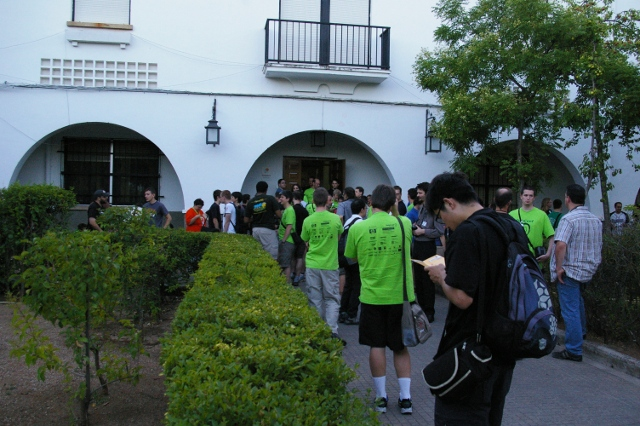
\includegraphics[width=5cm]{image200908/debconf9_venue.jpg}
  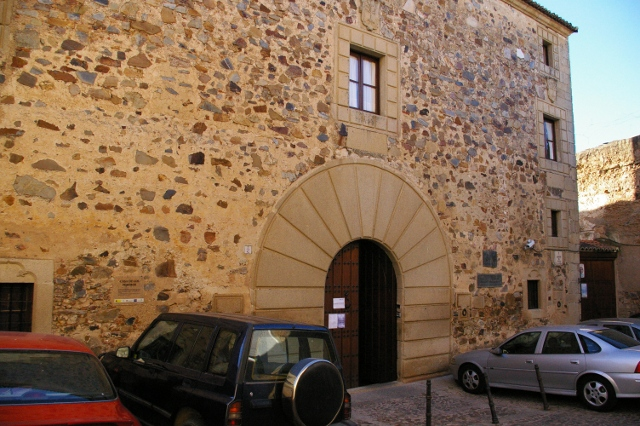
\includegraphics[width=5cm]{image200908/debconf9-fds.jpg}
\end{wrapfigure}
  会場は、エクストラマドゥーラの施設を借り切って開催されました。
  先に書いたとおり、宿泊施設が併設されており、4割の参加者は併設した宿泊施設から
  参加していました。もう片方の宿泊施設である Francisco de Sande は世界遺産である遺跡の
  中にあり、ゲームに出てきそうな宿でした。
  併設された宿泊施設には発表者やメイン開発者が泊まっており、ここでも格差社会が見え隠れしています。
  debconfの前にやっているdebcampと呼ばれるものがあり、こちらは開発が主体になっています。
  開発メインで行いたい人はdebcampから参加するとよいでしょう。
  \\

\begin{itemize}
  \item Upper Talk Room: 	メイン用。250人ほど入ることができます。\\
	\begin{minipage}{0.4\hsize}
	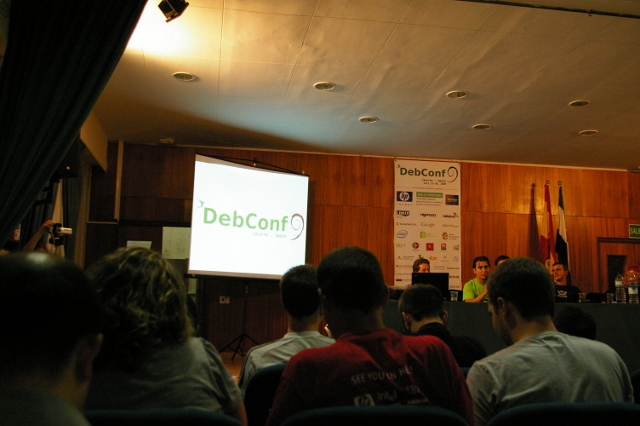
\includegraphics[width=0.8\hsize]{image200908/debconf9_main.jpg}
	\end{minipage}
  \item Lower Talk Room: サブ会場。50人ほど入ることができます。

  \item BoF Room\\
	BOF 用。30人ほど入ることができます。
        プレゼンテーション設備がないため、皆パソコンを開いてプレゼンテーション資料を見ていました。
	また、空調設備が貧弱なため、蒸し風呂状態でした。

  \item Hacklab 1/2 および 食堂: Hacklab はハック専用の部屋です。\\
	\begin{minipage}{0.4\hsize}
	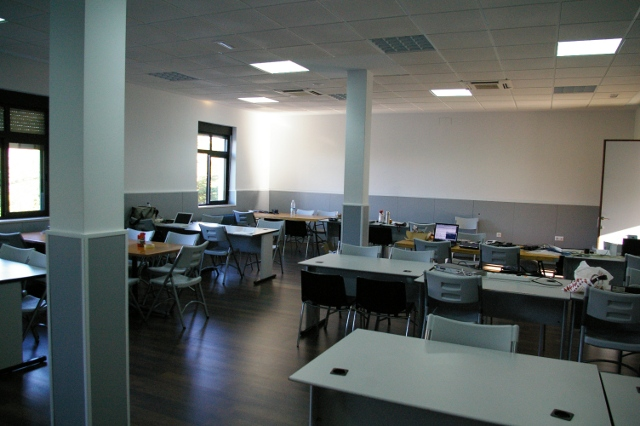
\includegraphics[width=0.8\hsize]{image200908/debconf9_hacklab.jpg}
	\end{minipage}
	\begin{minipage}{0.4\hsize}
	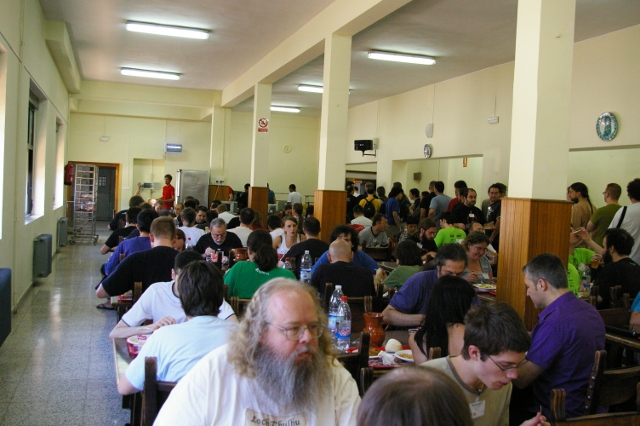
\includegraphics[width=0.8\hsize]{image200908/debconf9_diningroom.jpg}
	\end{minipage}

\end{itemize} 

\subsection{スケジュール}

23日のDebian Day で Debian Conference は開幕し、30日まで毎日いろいろな予
定が組まれていました。
27日だけはカンファレンス参加者で day-trip を実施しました。

\subsection{主となった討論}

\subsubsection{i18n関係}
今回も4回のi18nセッションが設けられ、リリースノート翻訳、DDTP、Wikiをつ
かった 翻訳などの検討が行われたようです。
DDTP翻訳パーティを検討されているようなので、日本からも参加できるようにし
たいところです。

\subsubsection{組み込み関係}
組み込み関係のセッションは全部で9つあり、組み込みからマルチアーキテクチャ
サポートなどが議論されました。

\subsubsection{Multiarch round table}
\subsubsection{Openmoko Buzz Fix Party}
カンファレス参加者に格安で提供されたOpenMokoのバグフィックスパーティ。
OpenMokoはフリーな携帯電話なのですが、日本では使えないので、購入はしませ
んでした。買った人に見せてもらったのですが、なかなかよさげです。Android
も動きますし。ただ、うまく携帯としてつかえないことがあるようで...(以下
略。
\subsubsection{Mer: Maemo Reconstructed}
Maemo のコミュニティ向け環境 Mer についての説明。
タブレットPC向けのようですが、N8XXやOpenMokoでも動作するようです。

\subsubsection{Scratchbox2 for crosscompiling debian}
Riku がメンテナンスしている Scratchbox2を組み込み環境でどのように利用す
るのか、という話。scratchboxでツールを作成し、scratchbox qemu のフロント
エンドとして利用したパッケージ作成ができるようになったので皆で使いましょ
う。

\subsubsection{uclibc and busybox}
uclibc と busybox Debianでどのようにサポートしたらいいのかという話。
emdebianで busyboxベースのdebian環境をサポートするために頑張っているよう
です。これらについての意見交換をしました。
sh4 もサポートに入る予定です。

\subsubsection{emdebian BoF}
毎回恒例になっている emdebianの進捗報告。
emdebianでは、Emdebian Grip と Emdebian Crush の2つのプロジェクトが
進行中。前者は busybox/uclibc ベースの debianを、後者は 現在のDebianをク
ロスコンパイルサポートするプロジェクト。emdebian-toolsができて、ある程度
ましになったけど、まだ不具合が多いので開発者募集中。apt-crossは依存関係
の実行がまだまだなので、今後力をいれて開発していくとのこと。
私からはsh4のサポートもするから強力しろ、と言っておきました。

\subsubsection{QEMU for Debian Developers}
aurel32 によるフリーのCPUエミュレータであるqemuの進捗状況と使い方につい
て。Debianでサポートしてるアーキテクチャのほとんどはqemuでサポートしてい
るのでマシンが手元になくてもデバッグできるよ、という話。
イメージも彼のWebサイトにあるので、mips や ppc などを試したい人はどうぞ。

\subsubsection{Crossbuilding on Debian for a derived distro}
既存のLinux組み込みシステムからDebianのシステムに移行した時の話とツール
の使い方、クロスコンパイルの方法についての話。
発表者のWookyは去年から会社が変わったのですが、システムをDebianに移行し
たので、そのときに行った方法を話していました。
CMakeでのクロスコンパイルが面倒だったようです。

\subsubsection{xcontrol}
Simon が毎年やっているxcontrolの話。debian/controlファイルを拡張してクロ
スコンパイルパッケージや、バックポートのサポートを容易にしましょうという
セッション。前回から進展があったのかは不明です。

\subsection{ツール関係}

\subsubsection{News on Debian Autobuilding}
buildd の現状と問題点の報告。
dep-wait、failedの遅延への対応や、パッケージプライオリティに対応したビルドについ
て議論されました。

\subsubsection{Trust is good, control is better}

パッケージのインストール、アンインストールのチェックができるpiupartsの進
捗報告。HPのマシン2台を使って、すべてのパッケージのチェックを定期的に行っ
ています。これにより、次期リリースではパッケージのインストール、アンイン
ストールが問題なくできるようになるでしょう。

\subsubsection{Using FOSSology for license analysis in Debian} 

tbm によるコードライセンス解析ソフトの話。deb, rpm,tarボールなどをリポジトリに食
わせライセンスの構文解析を行った結果をDBにまとめているとのこと。
ライセンスとCopurightがどのように変化していったのかまで調査できるようで
す。デモをしていましたが、ちょっと動きは遅いかな。
今後に期待です。\url{http://fossology.org/}

\subsubsection{not your grandpa's debhelper}

Joeyによるdebhelperの解説。debhelperはdh\_\*のプログラムを提供しますが、
これらをまとめたコマンド dh を作りましたという話。
dh を使うとdebian/rules を以下のようにまとめることができます。
\begin{commandline}
#!/usr/bin/make -f
%:
  dh: $@
\end{commandline}
各ターゲットもオーバーライドすることができて、override\_dh\_xxxx を作成し
ておくと呼ばれるようになります。dh 勉強会とかやりたいですね。

\subsubsection{UDD: Ultimate Debian Database}
% From http://kmuto.jp/d/index.cgi/travel/20090726-spain.htm
Debian/Ubuntuのパッケージ情報やpopcon情報、debtags、LDAP、アップロード履
歴、DDTP、testingミグレーション、バグ、NEWキュー、lintian、スクリーンショッ
トURL等々といった情報を全部PostgreSQLデータベースに突っ込んでデータマイ
ニングしてみました、というお話。
merkelやaliothでも試せる。


\subsubsection{pam-auth-update: manhandling debconf for fun and profit}
       squeezeから新しく導入された、pam-authの設定ツールです。今までは、
       /etc/pam.d/以下を手動で設定していましたが、/usr/share/pam-configs 以下の
       テンプレートを使い、postinst, prerm の中で、pam-auth-update コマンドを実
       行することで簡単に pam-auth の設定をできるようになります。3rd party 製の
       ツールも、これに則れば簡単に導入出来るようになるので、ユーザにとってもと
       てもメリットが大きいでしょう。Sid の環境では、次のファイルが既にこの制御
       下にあるようです。
 \begin{itemize}
  \item /etc/pam.d/common-account
  \item /etc/pam.d/common-auth
  \item /etc/pam.d/common-password
  \item /etc/pam.d/common-session
 \end{itemize}


\subsubsection{Changing the default system shell}
       デフォルトシェル /bin/sh をなぜ変えるのか?ポリシーもあるようです
       が、切り替える一番の動機としては、遅いからだということを言ってい
       ました。bash で記述されたものは約800あるうち、fix 済みのものは
       160 だそうです。bash を検出するには、devscripts, lintian, archive
       rebuilds, piuparts, ユーザの報告があるそうです。最終的には自分で
       判断して bash にするのをやめ、dash を選択するようにしてほしいと言っ
       ていました。

\subsubsection{DDE, Debian Data Export}
      Debian に関する情報を HTTP プロトコルで取得することができる
      RESTful アプリケーションのようです。
      \url{http://dde.debian.net/dde} や
      \url{http://debtags.debian.net/dde} から、データを取得することがで
      きます。

\subsubsection{Libvirt: Hypervisor independent virtual machine management}
       libvirt という仮想マシンを扱うための API の話です。Debian 固有の話
       は特になく、libvirt の紹介をしていました。Debian でもちゃんと使え
       るようなので、ぜひ使ってみましょう。

\subsubsection{RFH maintaining big packages}
       iceweasel のパッケージメンテナの Mike さんの BOF。iceweasel, OOo
       では、どうやってユーザや開発者をより多く巻き込んでいくか、活動を
       宣伝していくか、という点で議論が交わされました。

\subsection{リリース関係の話}
\subsubsection{Keynote from the Release Team}
Release team によるキーノート。Debianからのニュース
\url{http://www.debian.org/News/2009/20090729}でも流れているように
この場で、次期安定版であるSqueeze のフリーズとタイムベースリリースの話が
出ました。うまく行くか不安ではありましたが、その場ではいけるんじゃね?とい
う空気になっていました。(案の定、MLではフレームになっていますが。)

\subsubsection{GPGサイン}
Debconf9開催前にDSAの脆弱性が発覚し、これにより新しいGPG鍵を作成する
必要がでてきました。新しく作成した鍵を使って開発者同士で鍵サインをする必要が
出てきたため、今回のDebconfではGPGサインが活発に行われました。
今回のポイントはこれまでの事務的な手続きを反省して、Debconf開始に際してセッションを開き、
チェックサムの検証を行って、あとは好きなときにちゃんと相互におしゃべりをしながらサイン交換しましょうということがとても重要だったと思います。
名札にGPG鍵リスト上で割り当てられた番号が書かれていて、やりとりを促進するようにもなっていました。おかげで我々は29日夜のサインパーティに出られないながらも、
hacklabや食事どき、デイトリップの最中などいろいろな場面で多数サイン交換ができました。

武藤さん、岩松は40名ぐらいの参加者と交換することができました。



\subsection{Daytrip}

\begin{wrapfigure}{r}{5cm}
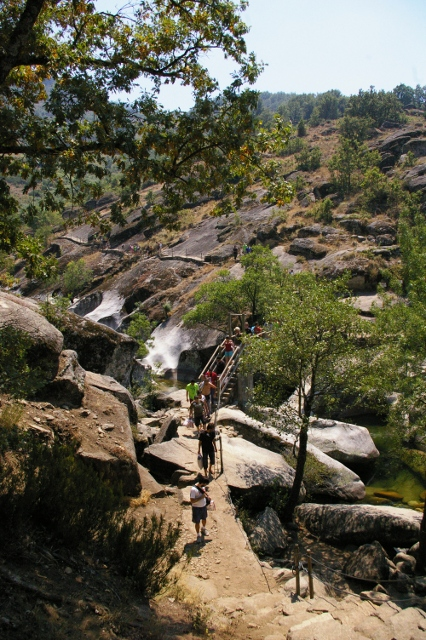
\includegraphics[width=5cm]{image200908/debconf9_daytrip.jpg}
\end{wrapfigure}

Debconf では一日、参加者で旅行をするというイベントがあります。今回の
Debconfでは 会場からバスで2時間ほど移動したところにあるエクストラマドゥーラ州が
運営しているキャンプ場に移動し、そこから1時間ほどハイキングをしました。
ハイキングの先には、自然でできたプール(Natural Pool)があり、そこで皆で泳いだり飛び込んだり、
滝に打たれていました。一部溺れかけてた人もいたようですが、皆無事だったようです。
4時間ほどそこで遊んだ後、別の場所に移動し、みんなでビールを飲みました。
そこにも川をせき止めたプールがあるのですが、皆のグランパであるJoeyが足を
ざっくり切ってしまうイベントが発生し、救急車が呼ばれるハプニングがありました。

\subsection{Debconf11}
Debconf11 はボスニアとドイツが立候補ししました。
ドイツはまだ場所が決まっていないようですが、今年中に場所を確定させるよう
です。ソマリアはトランジットが面倒ですが、開催地は空港から数キロのところ
にあり、そんなに困らないように感じました。
ドイツはDebian開発者が一番多い国で、Debconfチーム(orga)のメンバも多いた
め、ドイツ濃厚な気がします。

\subsection{今回のDebconf参加によるハックの成果}
\subsubsection{武藤さん}

ツアーコンダクターとして、マドリード観光や現地での皆さんの安全・食事探しに取り組みました。

\begin{itemize}
\item ドラゴンクエストIX\\
  出発時には最初の村を出るところでしたが、移動時間中だけで遊んでいたにもかかわらず、成田に戻る飛行機ではラスボスと戦っていました。全滅してしまったのでもう少し経験を重ねたいと思います。
\item フリーソフトウェアマップの翻訳\\
  スペインでフリーソフトウェアの活動を進めているGNUプロジェクトメンバーのRene Merouに頼まれて、彼らの作っているフリーソフトウェアマップを日本語に翻訳しました。政府機関にフリーソフトウェア採用を働きかけるなど、活発な活動をしているそうです。
% image200908にmap-ja.svg、map-ja.pngとしてコミット。どうリンクするとよい?
	\begin{minipage}{0.4\hsize}
	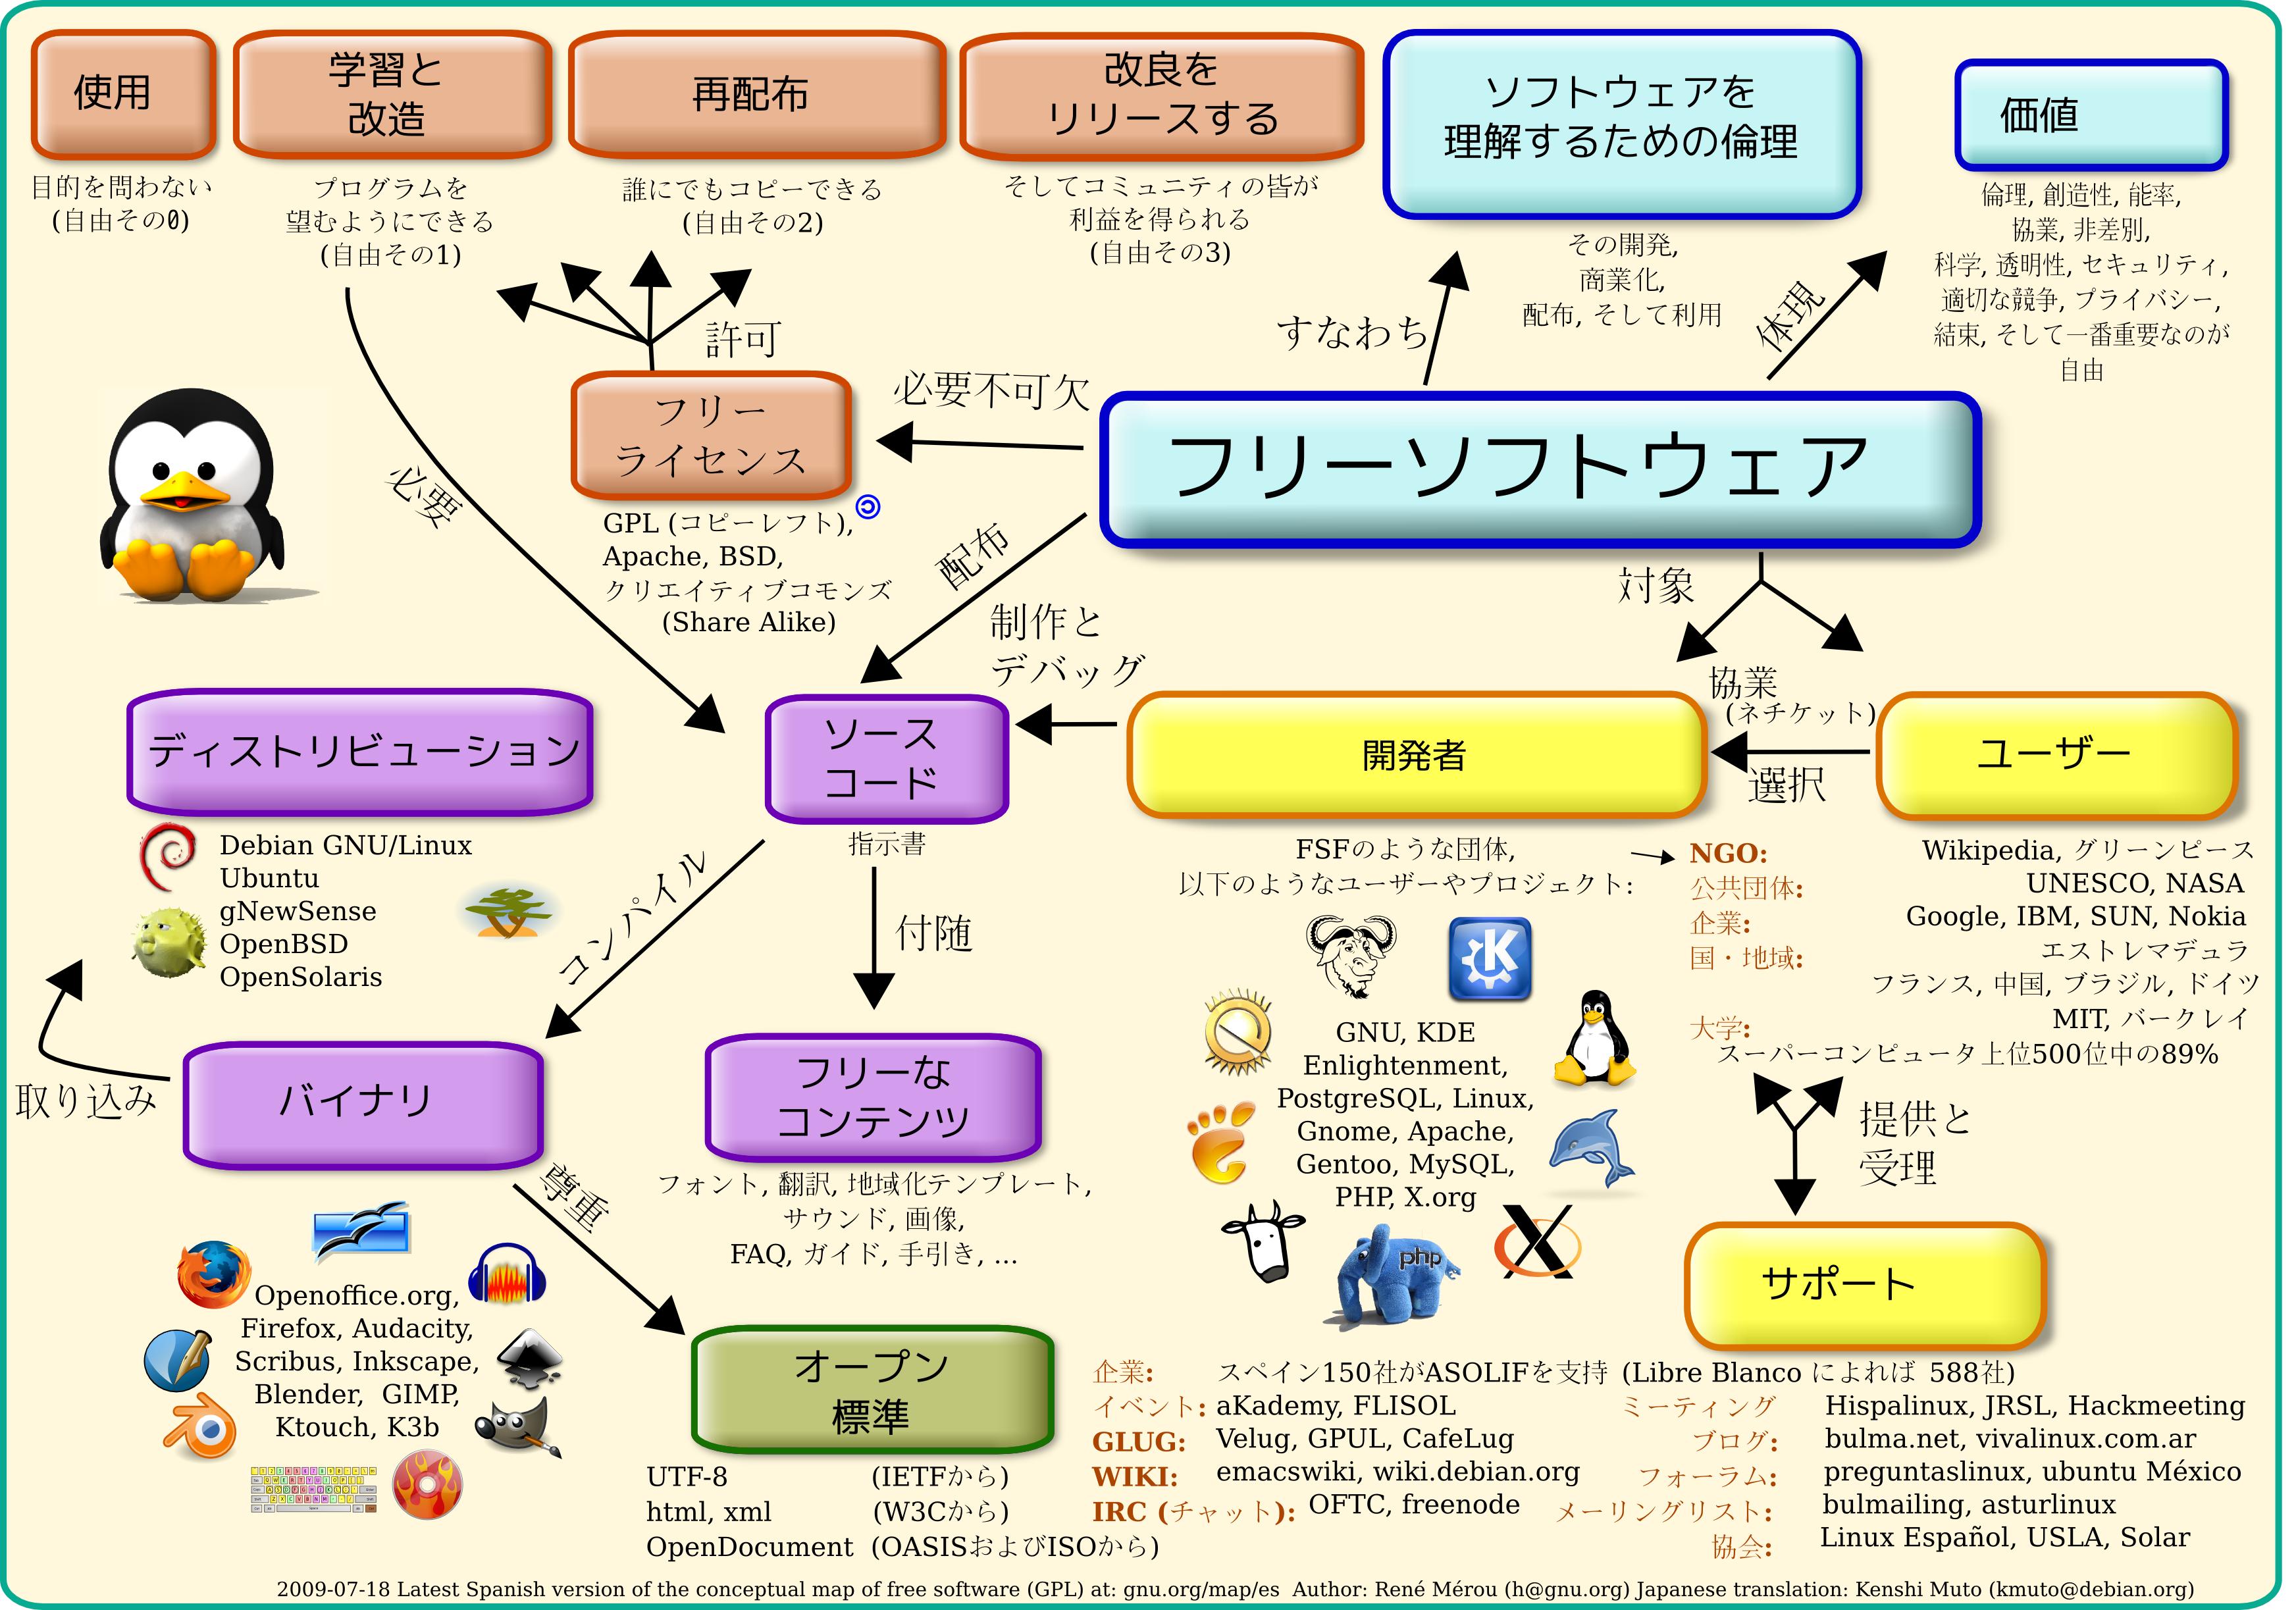
\includegraphics[width=2.0\hsize]{image200908/map-ja.png}
	\end{minipage}

\item ハードウェア互換性リストとハードウェアサポートページの友好関係構築\\
  Debianのハードウェアサポートの情報を収集してWiki(http://wiki.debian.org/HardwareDatabase, http://wiki.debian.org/DeviceDatabase/PCI など)にまとめているFranklin Piatに会って、私のDebian HCL(http://kmuto.jp/debian/hcl/)とどのような協業ができるかを話し合いました。まずは彼のUSBデータベースの成果を生かして、lsusbコマンドを貼り付けることでUSBのサポート情報を表示するようにHCLを拡張できるかを検討することになりました。
\item 国際化チームミーティング\\
  恒例の国際化チームミーティングは期間中4回開催され、WikiやDDTPについて議論がなされました。SqueezeではリリースノートをWikiベースで制作・編集するというトライアルが実施されます。Wikiのように変動の激しいものを翻訳するための手法として、poフォーマットに変換してパラグラフ単位で作業できるような手法も実施予定です。Debianのパッケージ説明翻訳機構のDDTPについても、多数の改善提案が出されました。パラグラフ単位でのマッチングやfuzzyマーキング、一般翻訳者を統轄するコーディネータという役割および特権を用意して一括置換や管轄する翻訳メンバーへの一斉連絡といった機能が追加される見込みです。日本のDDTP翻訳チームでも、いずれどなたかにコーディネータに立候補いただくことになると思われます。
\item 講演レポート\\
  各講演内容については
  http://kmuto.jp/d/index.cgi/travel/20090722-spain.htm,
  http://kmuto.jp/d/index.cgi/travel/20090724-spain.htm,
  http://kmuto.jp/d/index.cgi/travel/20090726-spain.htm,
  http://kmuto.jp/d/index.cgi/travel/20090728-spain.htm
  に短いながら報告しています。詳細についてはDebianの関連メーリングリストやDebconfサイトで掲載予定のビデオなどを参照してください。
\end{itemize}

3年ぶりの参加でしたが、新旧の友人たちと語らい、GPGサイン交換し、Debconf初参加者にDebconfを体感してもらい、国際化チームミーティングでup-to-dateな情報を得る、と当初の目的はいずれも達成できました。充実したカンファレンスだったと思います。

私自身は今後徐々にDebianに関する活動のペースを落としていくつもりなので(すでにだいぶ落ちてしまってはいますが)、特にDDTP関係者のDebconfおよび国際化チームミーティングへの参加を望みます。

\subsubsection{山根さん}

 兎に角、「参加することに意義がある」と言うことで参加してみました。初海外だったのでドキドキものです。色々と皆さんに助けていただきました。

\begin{itemize}
 
 \item po-debconf 訳\\
       多少は fuzzy, unstranslated を潰しました。
 \item フォントパッケージのライセンス確認\\
       日本語フォントについて、何故かスペインについてからupstreamに確認を取り始める私。
       「OFLだよ」「完全にフリーです、著作権も行使しません」との返答を得ました。
       パッケージにするのはdescriptionとdefoma-hintsファイルの作成が待ってますが…
 \item 参加レポート\\
       これとは別にまた少しだけ書いておこうと思います。
 \item GPG keysign\\
       15、6人ほどと鍵交換したはず。caff便利なんですね。そのうち使い方とかまとめたいかも。
 \item java policy 訳 review\\
       帰りの飛行機で半分ほどをレビューしました。何故。
\end{itemize}

 逆に課題としてもらってきたのは「英語英語英語〜」ですね。かなり精進が必要な模様です。

\subsubsection{前田さん}

数ヶ月溜まっていたタスク、問題を ToDo として取り組みました。

\begin{itemize}
 \item MacBook 5,2 の使えないデバイスを使えるようにする\\
       所有している MacBook は 2008 later モデル(通称 MacBook 5,2)ですが、
       DebConf に行く前に以下のような問題を抱えていました。

       \begin{itemize}
	\item 無線 LAN を使えない \\
	      Broadcom bcm4322 が搭載されており、b43 で将来的にはサポー
	      トされるらしいのですが、現状では Broadcom が提供している
	      STA ドライバを使用するしかありません。ただし、普段、
	      vanilla kernel の最新 stable を使用していると、このデバイ
	      スドライバをビルドできない、という問題があります。スペイン
	      から Twitter でつぶやいていたら、Gentoo の松鵜さんに、
	      Gentoo のパッチを使ってみては、と教えていただき、x86用のパッ
	      チを参考に、amd64(x86\_64) 用にコードを書き直したところ、
	      正常に無線 LAN を使えるようになりました。

	      実は Debian に既に Broadcom-sta ドライバ用のパッケー
	      ジがあり、これを使うと上記の問題は既に解決されている、とい
	      うオチもついてました。\footnote{broadcom-sta-common,
	      broadcom-sta-source パッケージ。i386 用にはバイナリパッケー
	      ジもあるようです。}
	\item 音が出ない \\
	      サウンドデバイスは認識しているものの、音が出ない、という現
	      象にハマっており、/etc/modprobe.d/alsa-base.conf の設定を
	      しなおすことでシステムブート時に音が出るようになりました。

	      が、これが非常にけたたましいビープ音で、イヤホンジャックに
	      イヤホンを挿してもなりやまず、Hacklab1 内でかなり顰蹙(ひん
	      しゅく)を買ってしまいました…。orz

	      帰国してから再設定したのですが、再び音が出なくなり、四苦八
	      苦中です。
	\item iSight が対応していない \\
	      isight-firmware-tools が、MacBook 購入時(2009年5月末)では
	      対応していなかったのですが、久しぶりに実行してみたら何もす
	      ることなくあっさりファームウェアを抽出でき、使えるようにな
	      りました。
	\item ACPI を有効にすると起動できない \\
	      この問題は未だ解決しておらず、ACPI を無効にするためバッテ
	      リー駆動の場合、残量が分からないとか、正常に電源を切れない
	      ため reboot ができず必ず shutdown しないといけないとか、ハ
	      イバネーションを行うと、復帰時に ACPI を有効にしたときと同
	      様に画面がブラックアウトして固まってしまう、という問題があ
	      ります。
	      
	      DebConf で MacBook を使っている人に聞いてみようかと思って
	      いたのですが、同じ世代の MacBook を使っている人が少なく、
	      持っていても Mac OS X を使っているので、断念しました。

	      ACPI の ML で聞いてみる予定です。
       \end{itemize}

 \item Java Policy の翻訳 \\
       4月の Debian 勉強会のネタとして、Java Policy を読んでみましたが、
       中途半端なところで翻訳を中断していました。再開するにあたり、PO 形
       式で整形し直し、未翻訳の部分の翻訳を完了し、debian-doc に投稿しま
       した。

       レビューコメントをやまねさんに頂いたのですが、帰国してから飼いは
       じめたネコに夢中で再び停滞しているので、今回の勉強会後に確認し、
       修正後、Java Policy のMLへの連絡及び、java-common パッケージのBTS
       を行う予定です。

 \item GanttProject のパッケージ化 \\
       ソースコードの入手方法が分からず、放置していたのですが、
       Subversion のリポジトリがあることに気づいたので、ドキュメントに沿っ
       てビルドしてみたところ、OpenJDK では正常に動くことを確認しました。

       他の Java 開発環境でのビルド、動作確認後、deb パッケージ化を行う
       予定です。

 \item Termtter のパッケージ化事前調査 \\
       jugyo さんが中心になって開発されている Twitter のターミナルクライ
       アントがあります。iceweasel の extention である twitterfox の使い
       勝手がいまいちなのと、ちょうど DebConf9 中に動作がおかしくなり、
       有効にしていると iceweasel ごと busy になってしまうので、切り替え
       ることにしました。使い勝手がよければ、deb パッケージにしてしまお
       うと考え、KVM環境で検証してみたところ、rubygems で必要なライブラ
       リを導入し、既に deb パッケージで導入済みのライブラリを無視してし
       まいます。

       今後の予定としては、その当たりの解決と、gems で導入されている deb
       パッケージになっていないライブラリ自体のパッケージ化の検討を行う
       つもりです。

 \item おまけ1。最近中古で買ったスーパーマリオブラザース DS をクリアしま
       した。クッパに息子がいるとは。またクッパはゾンビなってしまったのですね。

 \item おまけ2。最近、帰国後から飼い始めたネコですが、帰国後に引き取りに
       行くことが決まっていたので、事前にネコの健康本と、ネコの気持ちが
       分かる本を買っていきました。、帰宅後、熟読して帰ったらヨメにネコ
       博士と呼ばれるようになりました。
\end{itemize}

セッションにはいくつか参加しましたが、知らない内容を勉強するために出てみ
ても、英語の聞き取りがほとんど出来ないので、言っていることが分からないと
いう問題にぶち当たりました。そういう場合は、資料が頼りなのですが、事前に
配布されていないセッションも多く、おまけにスライドの文字が小さくて前の方
の席で眼鏡をかけても見えないようなセッションでは、非常に大変でした。





\subsubsection{岩松}
岩松は主に sh4 アーキテクチャ向けの開発を行いました。
\begin{itemize}
\item buildd hack\\
Debian / SH4 の buildd が動きはじめました。これにより、SH4向けバイナリが debian-ports.org
が取得できるようになります。
パッケージ作成の進捗は\url{http://www.debian-ports.org}から参照することができます。
\\
また、armel buildd メンテナである Riku と組み込み向けCPUで発生する問題を
どのようにフックしていくのか、意見交換を行いました。
\item debian kernel\\
tbm \footnote{元DPL, armのカーネルメンテナ} を捕まえて、debian kenrel configファイルのハックをしました。
sh4 向けカーネルサポートを一通りできました。

\item sh4 向けクロスコンパイラのサポートの打ち合わせ\\
gcc のクロスコンパイラサポートをしている zumbi と会話し、sh4 と uclibcのクロスコンパイラ
サポートの話をしました。gcc-4.4 ではうまく動作しないので修正したり、クロスコンパイルに
必要なパッケージを提供したりしていました。

\item defoma\\
defoma を ITA したままほったらかしにしていたので、CPAN adminをつついて、
バグのある CPANの乗っ取りを再開しました。CPANはやりとりが面倒くさいので新しい
ソフトウェアを作成したほうが早そうです。

\item Linux kernel/ U-boot \\ 
こっちに来ている間にもパッチが飛び交っているのでメールのチェックとパッチ
の査読をしていました。

\item speedstep-centrino
自分の使ってるMacBookはCoreDuoなので、speedstep-centrinoが使えるはずなの
ですが、モジュールのロードに失敗します。CPUマニュアルを斜め読みして対応
してみました。


\end{itemize}
\subsection{次回のDebconf}
次回のDebconf10は 米国のニューヨークで開催される予定です。
一部の日本人が日本での開催を再度目論んでいるようです。
スポンサーとか会場情報募集中。
\clearpage

%\printindex

\cleartooddpage

\vspace*{15cm}
\hrule
\vspace{2mm}

\includegraphics[width=2cm]{image200502/openlogo-nd.eps}
\noindent \Large \bf Debian 勉強会資料\\ \\
\noindent \normalfont \debmtgyear{}年\debmtgmonth{}月\debmtgdate{}日 \hspace{5mm}  初版第1刷発行\\
\noindent \normalfont 東京エリア Debian 勉強会 (編集・印刷・発行)\\
\hrule


\end{document}
